\section{引力常数$G$}

在上节的讨论中,我们并没有给出式\eqref{eqn:04.02.05}中的$ \alpha ' $值。因
为在解决这个问题的过程中,最终把$ \alpha ' $消去了,式\eqref{eqn:04.02.10}中不
含$ \alpha ' $。下面我们来讨论$ \alpha ' $应是什么。

% 131.jpg
\clearpage
由式\eqref{eqn:04.02.05},地球对月亮的力为
\begin{equation}\label{eqn:04.03.01}
  F _ { \text{地} \to \text{月}} = m _ {\text{月}} \frac { \alpha ' } { l ^ { 2 } }
\end{equation}
反过来,根据万有引力是普适的,月亮对地球的引力应当有如下
的形式
\begin{equation}\label{eqn:04.03.02}
  F _ { \text{月} \to \text{地}} = m _ {\text{地}} \frac { \alpha '' } { l ^ { 2 } }
\end{equation}
其中$ \alpha '' $是和月亮有关的常数。根据牛顿第三定律,$F _ { \text{地} \to \text{月}}$与$F _ { \text{月} \to \text{地}}$
大小相等,即
\begin{equation*}
  \frac { \alpha ' } { \alpha '' } = \frac { m _ \text{地} } { m _ \text{月} }
\end{equation*}
因此,其解为
\begin{equation*}
  \alpha ' = G m _ { \text{地} } \qquad
  \alpha '' = G m _ { \text{月} }
\end{equation*}
这样,式\eqref{eqn:04.03.01}、\eqref{eqn:04.03.02}两式可统一为
\begin{equation}\label{eqn:04.03.03}
  F = \frac { G m _ { \text{地} } m _ { \text{月} } } { l ^ { 2 } }
\end{equation}

根据引力是普适的观点,任何具有质量$ m_1 $和$ m_2 $、相距$ r $的两
个质点之间的引力,总是沿着两质点的连线方向,其大小为
\begin{equation}\label{eqn:04.03.04}
  F = \frac { G m _ { 1 } m _ { 2 } } { r ^ { 2 } }
\end{equation}
式中$ G $是对所有质点都具有相同数值的普适常数,称为万有引力
常数。这就是牛顿的万有引力定律。

确定万有引力常数$ G $的数值,就要测量两个已知质量的物体
间的引力。1798年,卡文迪许作了第一个精确的测量。他用的扭
秤如图\ref{fig:04.04}~所示。其中两个质量均为$ m $的小球固定在一轻杆的两
端,再用一根细丝将这个杆水平悬挂起来,每个质量$ m $附近各放置
一个质量为$ M $的大球。根据万有引力定律,当大球在位置$ A , B $
时,由于小球受到吸引力,而对悬杆产生一力矩,使其产生转动。\\~\\
% 132.jpg
引力力矩最后被悬丝力矩所平衡。悬丝扭转的角度$ \theta $可以通过小
镜所反射的光来测定。如果已知大球与小球的质量和它们相隔的
距离以及悬丝的扭转常数,就可由测得的$ \theta $值来计算$ G $。
\begin{figure}[h]
  \centering
  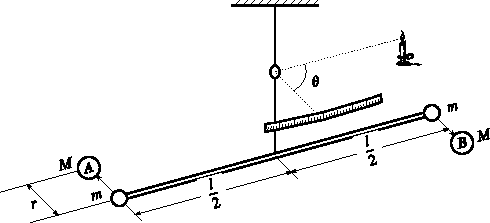
\includegraphics{figure/fig04.04}
  \caption{测量引力常数所用的扭秤}
  \label{fig:04.04}
\end{figure}

还曾用过以下几种方法测量引力常数$ G $。

\textsf{1.天平法}

如果天平两边各有质量$ m $,达到平衡。若再将一大质量$ M $放
在某一$ m $之下,由于引力的作用将破坏这个平衡,必须将另一端
之$ m $增加为$  m + \delta m $才能保持平衡由$ \delta m $及其他天平参数,即可求
出$ G $。

\textsf{2.扭秤周期法}

这种方法的原理是扭秤的摆动周期在引力的作用下会发生变
化。如图\ref{fig:04.04}~所示,若将一个大质量$ M $放在横杆方向,则其摆动周
期将缩短;若$ M $放在垂直于横杆的方向,周期将增加,由周期差
别可以确定$ G $。

\textsf{3.扭秤共振法}

在图\ref{fig:04.04}~中,把两个$ M $也作为一扭秤的两端悬挂起来,这样
形成两扭摆系统,一个扭摆的质量小($ m $),一个质量大($ M $)  。当
$ M $摆动时,由于引力的作用也将引起$ m $摆动。当调节两个摆的周
% 133.jpg
期相同时,$ m $摆与$ M $摆的振幅之比是正比于$ G $的。因而,由摆的
振幅即可定出$ G $。

用这些方法测得的$ G $值列于表4.2中,从表中看到,从卡文迪
许第一个实验以来,已经有近二百年了,但关于$ G $值的实验精度
进步不大。这是目前测得最不精确的一个物理常数。原因是实验
很难做,一方面引力是四种基本相互作用中最弱的一种;另一方
面,引力是万有的,不能屏蔽,这就意味着干扰很多,不容易排
除。

$ G $的单位是牛顿\cdot 米\.$^2$/千克\.$^2$。关于单位的确定,我们在下节
中作些一般的讨论。
\begin{table}[h]
  \caption{}
  \label{tab:04.02}
  \zihao{-5}
  \begin{tblr}{cell{1}{1-Z}={c,m},colspec={l|c|l|Z},colsep=0.8em}
    \toprule
    \SetCell{c}作\hspace{4em}者 & 年份 & \SetCell{c}方\hspace{4em}法& {{{$G  \times 10^{-11}$\\牛顿$\cdot$米\textsuperscript{2}/千克\textsuperscript{2}}}} \\
    \midrule
    Cavendish                       & 1798 & 扭秤偏转                  & 6.754                                  \\
    Poynting                        & 1891 & 天平偏转                  & 6.698                                  \\
    Boys                            & 1895 & 扭秤偏转                  & 6.658                                  \\
    Braun                           & 1895 & 扭秤偏转和周期            & 6.658                                  \\
    Heyl                            & 1930 & 扭秤周期                  & 6.678                                  \\
    Zahradnicek                     & 1933 & 扭秤共振                  & 6.659                                  \\
    Heyl and Clirzanowski           & 1942 & 扭秤周期                  & 6.668                                  \\
    Rose                            & 1969 & 加速度                    & 6.674                                  \\
    \bottomrule
  \end{tblr}
\vspace{-0.8em}
\end{table}
